% Mid-semester evaluation report: Group 59, Project 1.
% ---------------------------------------------------------------------------
% This file is a SKELETON. Headings, figures, tables, code listings and the
% bibliography are filled in from the artifact. Every paragraph marked \todo
% has to be written by the group: the course prohibits AI-written reports.
% Each \todo is followed by LaTeX comments (%) listing the verified facts and
% numbers from results/ and docs/MEASUREMENT_NOTES.md that the paragraph can use.
% Build: cd report && pdflatex midsem_report && bibtex midsem_report && pdflatex midsem_report && pdflatex midsem_report
% ---------------------------------------------------------------------------
\documentclass[11pt,a4paper]{article}
\usepackage[margin=2.2cm]{geometry}
\usepackage{graphicx}
\usepackage{booktabs}
\usepackage{listings}
\usepackage{xcolor}
\usepackage{float}
\usepackage{caption}
\usepackage{amsmath}
\usepackage[hidelinks]{hyperref}
\usepackage{url}

\newcommand{\todo}[1]{\textcolor{red}{\textbf{[TODO: #1]}}}
\lstset{basicstyle=\ttfamily\footnotesize, language=C, breaklines=true, frame=single, columns=fullflexible, keepspaces=true}
\graphicspath{{figures/}}

\title{Sparse-Aware RISC-V Vector Architecture for High-Performance Computing\\
\large Mid-Semester Evaluation Report --- Project 1, Group 59}
\author{Sakshat Sachdeva (2023474) \and Ansh Verma (2023101)}
\date{\today}

\begin{document}
\maketitle

\begin{abstract}
\todo{4--6 sentences: what was built, what was measured, the one-line finding, what comes next.}
% Facts: three kernels (scalar CSR, dense RVV GEMV, CSR RVV SpMV) on Spike+pk; 10 sparsity levels x
% 3 patterns x 3 VLENs = 270 runs, all PASS; dense cost is flat, CSR cost falls with sparsity but hits a
% floor; avg vector length drops from 16 to 1.95 lanes at 99% sparsity (VLEN=512).
\end{abstract}

\section{Problem and Motivation}
\todo{Why vector hardware loses efficiency on sparse data; why SpMV is the chosen workload; what the project will build by the end-evaluation.}
% Spec text to paraphrase, not copy: "many vector elements may be zero or inactive; processing them
% results in unnecessary computation, vector-register usage and memory traffic." SpMV is the primary
% workload named in the project description.

\section{Background}
\subsection{The RISC-V Vector Extension}
\todo{VLEN, SEW, LMUL, VLMAX; vsetvl and strip-mining; tail policy; unit-stride vs indexed loads; reductions. Cite \cite{rvvspec}.}
% VLMAX = VLEN/SEW * LMUL. We use SEW=32, LMUL=1, so VLMAX = 4, 8, 16 for VLEN = 128, 256, 512.
% vsetvl returns min(avl, VLMAX) on Spike. Indexed load used: vluxei32 (byte offsets, unordered).
% Reduction used: vfredusum (unordered sum).

\subsection{Sparse Formats and SpMV}
\todo{CSR (rowptr, colidx, vals); where the indirect access is; memory footprint of CSR vs dense; mention COO, ELL, SELL-C-sigma briefly. Cite \cite{bell2009spmv,kreutzer2014sell}.}
% CSR bytes = 8*nnz + 4*(N+1) (float values, 32-bit indices); dense bytes = 4*N*N.
% Break-even at nnz = N^2/2, i.e. 50% sparsity.

\subsection{Existing Sparse-Aware Architectures}
\todo{Short survey, 1--2 sentences each, with citations you have actually read (see docs/READING\_LIST.md).}

\section{Experimental Setup}
\begin{table}[H]
\centering
\caption{Simulation environment.}
\begin{tabular}{ll}
\toprule
Compiler & riscv64-unknown-elf-gcc 16.1.0, \texttt{-O2 -march=rv64gcv\_zicntr -mabi=lp64d} \\
Simulator & Spike 1.1.1-dev (commit 609dbe0b) with proxy kernel pk (commit 9c61d298) \\
ISA string & \texttt{rv64gcv\_zicntr\_zvl\{128,256,512\}b} \\
Vector config & SEW = 32 (float), LMUL = 1, VLMAX = 4 / 8 / 16 \\
Matrix size & $N = 128$, seed 1 (also validated at $N = 37, 100$ and seeds 2, 3) \\
Sparsity levels & 0, 0.1, 0.2, 0.3, 0.4, 0.5, 0.8, 0.9, 0.95, 0.99 (target; actual value reported) \\
Patterns & uniform random, banded, $8\times8$ block \\
Metric & retired instructions (\texttt{rdinstret}) of the second call of each kernel \\
Correctness & relative error $< 10^{-3}$ against a double-precision Python reference \\
\bottomrule
\end{tabular}
\end{table}
\todo{One paragraph on the toolchain build (scripts/setup\_tools.sh), one on how a run works (make spike), one on what Spike can and cannot measure.}
% Spike is functional: rdcycle == rdinstret. No pipeline, no cache, no memory latency.
% A 16-element gather counts as one instruction, same as an add.

\subsection{Measurement Methodology}
\todo{Explain the warm-up call and why it is needed; explain how vec\_iters and avg\_vl are obtained.}
% pk maps pages lazily; the first touch of each 4 KiB page traps and the handler instructions
% (about 5100 per page) are counted by rdinstret. A_dense is 64 KiB = 16 pages.
% Table below: first vs second call, N=128, VLEN=512, uniform, sparsity 0.
\begin{table}[H]
\centering
\caption{Instructions retired by the first (cold) and second (warm) call of each kernel. $N=128$, VLEN = 512, uniform, sparsity 0.}
\begin{tabular}{lrrr}
\toprule
kernel & first call & second call & ratio \\
\midrule
scalar\_csr & 324036 & 149645 & 2.17 \\
dense\_rvv & 95383 & 13458 & 7.09 \\
csr\_rvv & 13712 & 13713 & 1.00 \\
\bottomrule
\end{tabular}

\end{table}

\section{Baseline Implementations}
\subsection{Dense RVV GEMV}
\lstinputlisting[firstline=16,lastline=34,caption={Dense GEMV with RVV intrinsics (src/kernels.c).}]{../src/kernels.c}
\todo{Walk through the loop: strip-mining with vsetvl, two unit-stride loads, vfmacc with tail-undisturbed, one reduction per row. Why \_tu is required.}

\subsection{CSR RVV SpMV}
\lstinputlisting[firstline=36,lastline=56,caption={CSR SpMV with RVV intrinsics (src/kernels.c).}]{../src/kernels.c}
\todo{Walk through: load column indices, shift to byte offsets, indexed gather of $x$, load values, vfmacc, reduction. Why the vector never crosses a row boundary and what that costs.}
% Both inner loops compile to 12 instructions per chunk (objdump -d bin/uniform_s0.0).
% Instruction model: dense = 12*N*ceil(N/VLMAX) + 9N + 18; CSR = 12*sum_rows ceil(nnz_row/VLMAX) + 11N + 17;
% scalar = 9*nnz + 17N + 13. Matches every row of results/vlen*/table.csv to within one instruction.

\subsection{Scalar Reference and Correctness Check}
\todo{Scalar CSR loop; the Python-generated reference; tolerance; why the vector result differs from scalar at the $10^{-5}$ level (unordered reduction).}

\section{Results}
\subsection{Instructions versus Sparsity}
\begin{figure}[H]
\centering
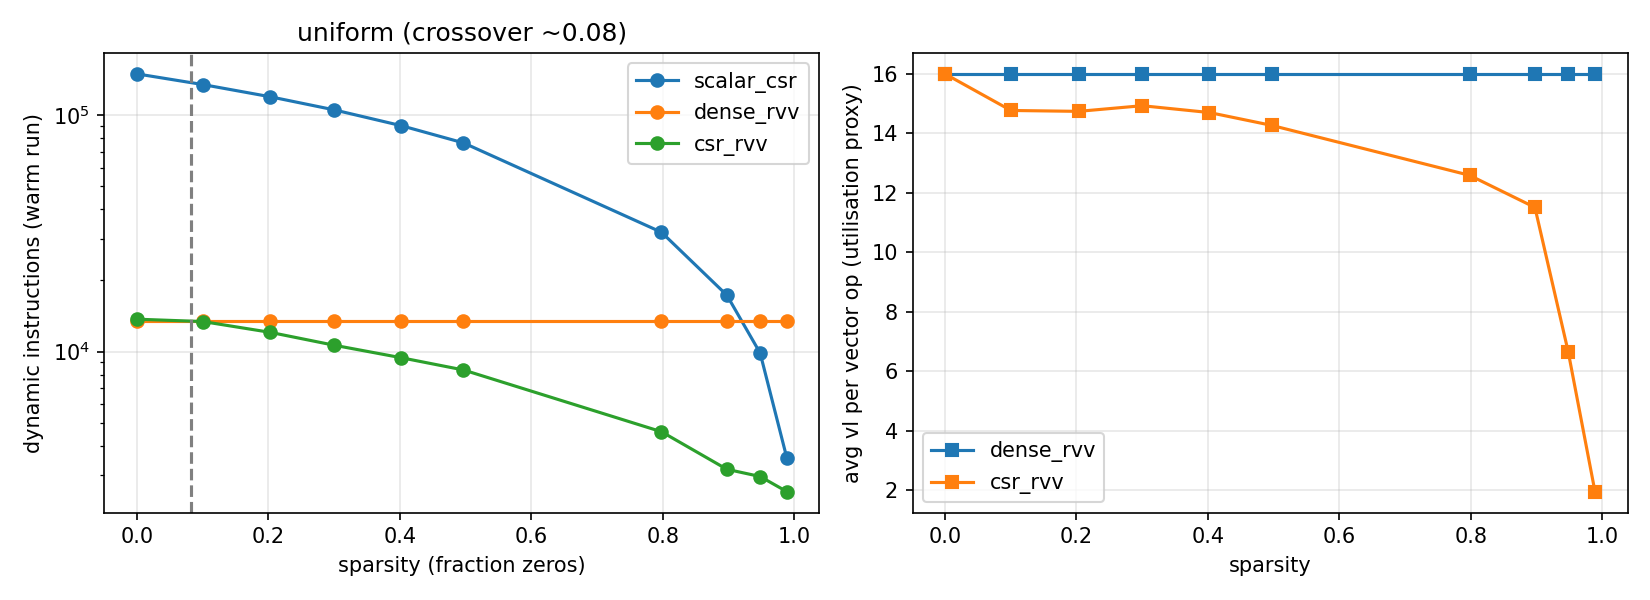
\includegraphics[width=\textwidth]{instret_vs_sparsity_uniform}
\caption{Uniform pattern, VLEN = 512. Left: retired instructions per kernel (log scale), dashed line marks the observed dense-to-CSR crossover. Right: average vector length per vector operation.}
\end{figure}
\begin{table}[H]
\centering
\caption{Uniform pattern, VLEN = 512, $N = 128$. Instruction counts of the warm call; avg vl is for CSR RVV.}
\begin{tabular}{rrrrrrrr}
\toprule
sparsity & nnz & scalar CSR & dense RVV & CSR RVV & avg vl & dense/CSR & scalar/CSR \\
\midrule
0.000 & 16384 & 149645 & 13458 & 13713 & 16.00 & 0.98 & 10.91 \\
0.100 & 14741 & 134858 & 13458 & 13401 & 14.77 & 1.00 & 10.06 \\
0.203 & 13056 & 119693 & 13458 & 12057 & 14.74 & 1.12 & 9.93 \\
0.300 & 11470 & 105419 & 13458 & 10641 & 14.93 & 1.26 & 9.91 \\
0.402 & 9792 & 90317 & 13458 & 9417 & 14.70 & 1.43 & 9.59 \\
0.497 & 8246 & 76403 & 13458 & 8361 & 14.27 & 1.61 & 9.14 \\
0.798 & 3311 & 31988 & 13458 & 4581 & 12.59 & 2.94 & 6.98 \\
0.897 & 1681 & 17318 & 13458 & 3177 & 11.51 & 4.24 & 5.45 \\
0.948 & 852 & 9857 & 13458 & 2961 & 6.66 & 4.55 & 3.33 \\
0.989 & 183 & 3530 & 13458 & 2554 & 1.95 & 5.27 & 1.38 \\
\bottomrule
\end{tabular}

\end{table}
\todo{Describe what the table shows. Do not interpret yet.}

\subsection{Effect of Sparsity Pattern}
\begin{figure}[H]
\centering
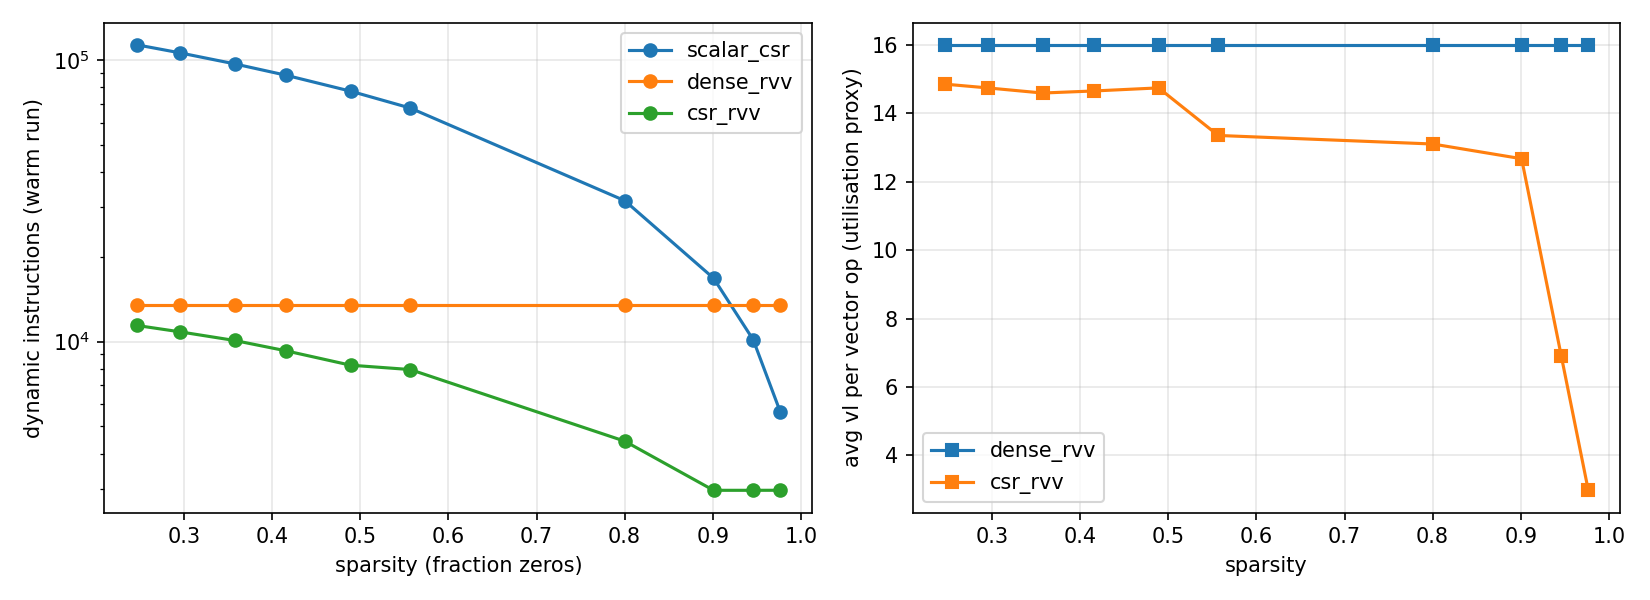
\includegraphics[width=\textwidth]{instret_vs_sparsity_banded}\\
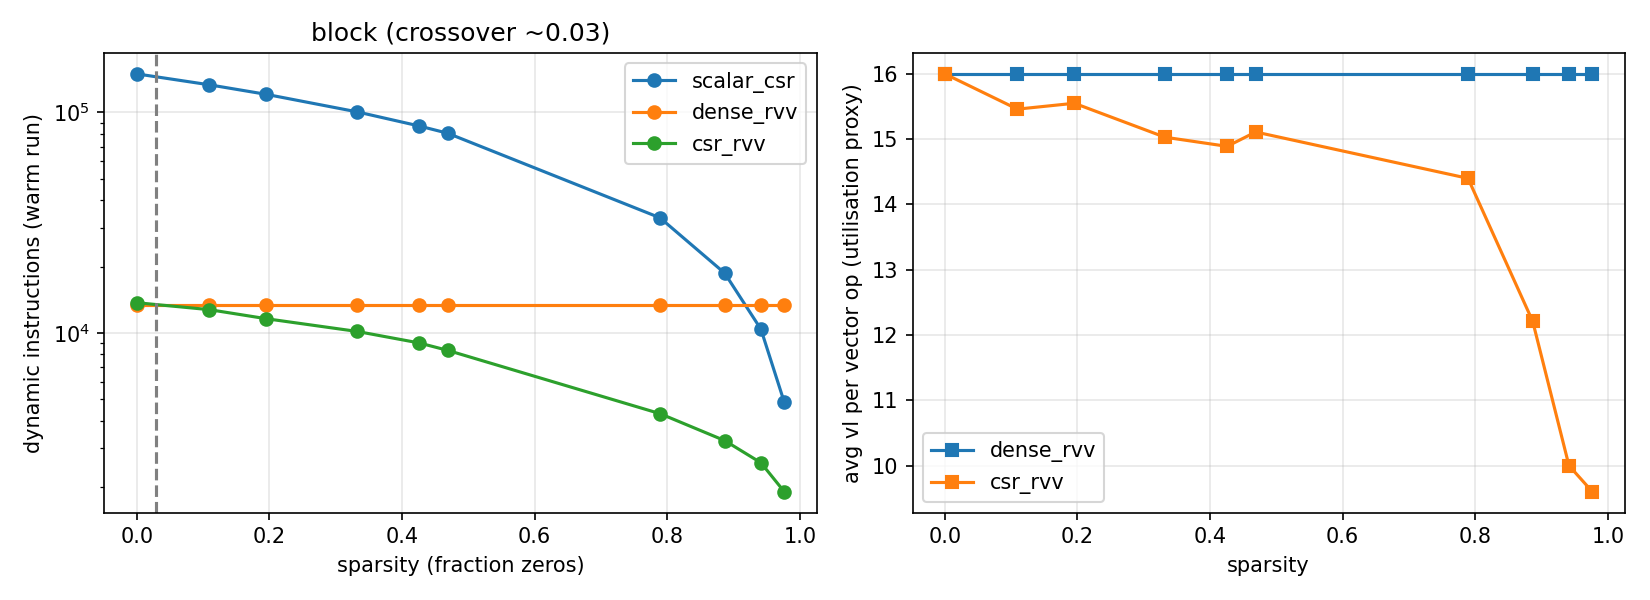
\includegraphics[width=\textwidth]{instret_vs_sparsity_block}
\caption{Banded (top) and $8\times8$ block (bottom) patterns, VLEN = 512.}
\end{figure}
\begin{table}[H]
\centering
\caption{Block pattern, VLEN = 512.}
\begin{tabular}{rrrrrrrr}
\toprule
sparsity & nnz & scalar CSR & dense RVV & CSR RVV & avg vl & dense/CSR & scalar/CSR \\
\midrule
0.000 & 16384 & 149645 & 13458 & 13713 & 16.00 & 0.98 & 10.91 \\
0.109 & 14592 & 133517 & 13458 & 12753 & 15.46 & 1.06 & 10.47 \\
0.195 & 13184 & 120845 & 13458 & 11601 & 15.55 & 1.16 & 10.42 \\
0.332 & 10944 & 100685 & 13458 & 10161 & 15.03 & 1.32 & 9.91 \\
0.426 & 9408 & 86861 & 13458 & 9009 & 14.89 & 1.49 & 9.64 \\
0.469 & 8704 & 80525 & 13458 & 8337 & 15.11 & 1.61 & 9.66 \\
0.789 & 3456 & 33293 & 13458 & 4305 & 14.40 & 3.13 & 7.73 \\
0.887 & 1856 & 18677 & 13458 & 3249 & 12.21 & 4.14 & 5.75 \\
0.941 & 960 & 10397 & 13458 & 2577 & 10.00 & 5.22 & 4.03 \\
0.977 & 384 & 4853 & 13458 & 1905 & 9.60 & 7.06 & 2.55 \\
\bottomrule
\end{tabular}

\end{table}
\begin{table}[H]
\centering
\caption{Banded pattern, VLEN = 512. Note the banded generator cannot reach sparsity below 0.25 at $N=128$ (band half-width is capped at $N/2$).}
\begin{tabular}{rrrrrrrr}
\toprule
sparsity & nnz & scalar CSR & dense RVV & CSR RVV & avg vl & dense/CSR & scalar/CSR \\
\midrule
0.246 & 12352 & 113357 & 13458 & 11409 & 14.85 & 1.18 & 9.94 \\
0.295 & 11554 & 106175 & 13458 & 10833 & 14.74 & 1.24 & 9.80 \\
0.357 & 10532 & 96977 & 13458 & 10089 & 14.59 & 1.33 & 9.61 \\
0.415 & 9578 & 88391 & 13458 & 9273 & 14.65 & 1.45 & 9.53 \\
0.489 & 8374 & 77555 & 13458 & 8241 & 14.74 & 1.63 & 9.41 \\
0.557 & 7264 & 67565 & 13458 & 7953 & 13.35 & 1.69 & 8.50 \\
0.800 & 3274 & 31655 & 13458 & 4425 & 13.10 & 3.04 & 7.15 \\
0.901 & 1622 & 16787 & 13458 & 2961 & 12.67 & 4.55 & 5.67 \\
0.946 & 884 & 10145 & 13458 & 2961 & 6.91 & 4.55 & 3.43 \\
0.977 & 382 & 5627 & 13458 & 2962 & 2.98 & 4.54 & 1.90 \\
\bottomrule
\end{tabular}

\end{table}

\subsection{Effect of Vector Length}
\begin{table}[H]
\centering
\caption{Uniform pattern: dense and CSR RVV instruction counts at VLEN = 128, 256, 512.}
\begin{tabular}{rrrrrrr}
\toprule
sparsity & dense V128 & CSR V128 & dense V256 & CSR V256 & dense V512 & CSR V512 \\
\midrule
0.000 & 50322 & 50577 & 25746 & 26001 & 13458 & 13713 \\
0.100 & 50322 & 46245 & 25746 & 24213 & 13458 & 13401 \\
0.203 & 50322 & 41145 & 25746 & 21669 & 13458 & 12057 \\
0.300 & 50322 & 36405 & 25746 & 19305 & 13458 & 10641 \\
0.402 & 50322 & 31413 & 25746 & 16797 & 13458 & 9417 \\
0.497 & 50322 & 26769 & 25746 & 14517 & 13458 & 8361 \\
0.798 & 50322 & 11949 & 25746 & 7089 & 13458 & 4581 \\
0.897 & 50322 & 7005 & 25746 & 4569 & 13458 & 3177 \\
0.948 & 50322 & 4581 & 25746 & 3285 & 13458 & 2961 \\
0.989 & 50322 & 2578 & 25746 & 2554 & 13458 & 2554 \\
\bottomrule
\end{tabular}

\end{table}

\section{Analysis}
\todo{Why dense is flat. Why CSR cost falls then floors. Why avg vl collapses. Why block keeps avg vl high. Why wider vectors stop helping. Where the crossover is and why the Spike crossover is a lower bound.}
% Numbers (VLEN=512, uniform): dense 13458 at every sparsity. CSR 13713 -> 8361 -> 3177 -> 2961 -> 2554
% at sparsity 0 / 0.5 / 0.9 / 0.95 / 0.99. avg vl 16.0 -> 14.27 -> 11.51 -> 6.66 -> 1.95.
% From 0.95 to 0.99 nnz drops 4.7x, instructions drop 1.16x. CSR floor = 11N + 12*(non-empty rows) + 17.
% At 0.99: VLEN128 CSR = 2578, VLEN512 CSR = 2554 (same). Scalar 3530 vs CSR 2554 (1.4x).
% Block at ~0.977: 1905 instr, avg vl 9.6. Banded at 0.977: 2962 instr, avg vl 2.98.
% Observed crossovers (instruction count): uniform 0.08, block 0.03 at VLEN512; 0.006 / 0.005 at VLEN128.

\section{Limitations and Failure Cases}
\todo{Spike is not a timing model; gather cost hidden; no cache model; small N; synthetic matrices only; first measurements were wrong and why (page faults, in-loop counters), see docs/MEASUREMENT\_NOTES.md.}

\section{Plan for the End-Evaluation}
\todo{Chosen mechanism (software format such as SELL-C-sigma, or a modelled hardware mechanism in Spike), timing model choice (Ara/Verilator vs gem5), second workload, metrics required by the spec, schedule and roles.}

\section*{Artifact}
Source, scripts, results and documentation are in the submitted archive \texttt{59\_1.zip}; see \texttt{README.md}. Representative result: \texttt{make spike N=64 SPARS="0.5 0.9" PATTERNS=uniform OUT=/tmp/demo}.

\bibliographystyle{ieeetr}
\bibliography{refs}
\end{document}
